%% LyX 2.0.0 created this file.  For more info, see http://www.lyx.org/.
%% Do not edit unless you really know what you are doing.
\documentclass[12pt,english]{article}
\usepackage[T1]{fontenc}
\usepackage[latin9]{inputenc}
\usepackage{subscript}
\usepackage{listings}
\usepackage{wrapfig}
\usepackage{graphicx}
\usepackage[usenames,dvipsnames,svgnames,table]{xcolor}
\makeatletter

%%%%%%%%%%%%%%%%%%%%%%%%%%%%%% LyX specific LaTeX commands.
%% Because html converters don't know tabularnewline
\providecommand{\tabularnewline}{\\}

\makeatother

\usepackage{babel}
\begin{document}

\title{\textbf{aML}\\
a-Mazing Language}


\author{Sriramkumar Balasubramanian (\textbf{sb3457})\\
 Evan Drewry (\textbf{ewd2106})\\
 Timothy Giel (\textbf{tkg2104})\\
 Nikhil Helferty (\textbf{nh2407})}

\maketitle
\pagebreak{}
\tableofcontents{}
\pagebreak{}

\section{Introduction}
A maze is a puzzle in the form of a series of branching passages through which a solver must a route. 
Actual mazes have existed since ancient times, serving as a means to confuse the traveler from finding
his or her way out. Since then, the idea behind mazes has been extrapolated to construct a set of 
puzzles designed to challenge people to solve or find the route.
 
While the concept of maze solving might seem too restricted, maze exploration in general can be 
extrapolated to other fields like Graph theory and topology. Apart from this, there exist more than one 
way to solve mazes, which has led to the rise of the time and space analysis of these approaches.  Also 
solving a maze can be likened to exploring a map which paves way for many practical uses of a language
for solving mazes.

Having justified the existence of a language to solve mazes, we now introduce AML (A-mazing Language) 
which can be used to solve mazes by feeding instructions to a bot which is located at the entrance to the maze at time 0.  The maze in question can either be defined by the user in the form of text files or can be randomly generated by the standard library functions. 
AML is designed to not only make the process of solving mazes easier to a programmer, but also to 
introduce programming to the common man through mazes. 

AML's design ensures the freedom of the user to implement many maze solving algorithms, while 
ensuring the ease of use of the language to traverse mazes. The language serves as an instruction set to 
the bot, hence the movement of the bot determines accessing of various data.  

\pagebreak
\section{Tutorial}
The syntax of aML is similar to a simplified version of Java, or C. The available instructions allow you to move a bot around a maze. You can define your own functions in order to program bots with complex behavior. aML will provide a simple Graphical User Interface of the bot navigating the maze (either randomly generated or provided in a .txt file).

aML has a limited set of data types for variables to take. The most basic types are integer, analogous to the Java int, and bool, like the Java boolean. A third, slightly more complex datatype is cell. This represents a cell in the maze. The programmer can't construct new cells as that would alter the maze, they can only set a cell variable equal to an existing cell of the maze in order to find out information about it. The fourth, and most complex datatype, is List<datatype> (such as List<integer>), which is a First In First Out List that behaves much like a linked list.

Users can define their own functions in aML. A function can either return a datatype (function x():integer) or be void and return nothing. Functions can be recursive (no looping constructs are offered). A special function is main, which must be void and parameterless. main is always the first function in any given program, and is the function that aML will call when the program is run.

\subsection{Making Your Own Maze}
If users wish to build a custom maze for the bot to navigate, then the maze text file must adhere to a certain format. The text file must be a sequence of integers delimited by whitespace. The first integer is the number of rows in the maze; the second, the number of columns. Then an integer follows for every cell in the maze: either a 0 for a "hole" (unwalkable), a 1 for a walkable cell, a 2 for the starting cell of the bot, and a 3 for a target cell for the bot (note it is possible to have multiple targets). The format can be clearly illustrated by the following example:
\\\\\\\\
\begin{center}
\begin{tabular}{c}
\begin{lstlisting}
5 6

0 1 1 1 0 0 
1 1 2 0 1 1
0 0 1 1 1 0
0 1 1 0 1 3
0 3 1 0 1 1         
\end{lstlisting}
\end{tabular}
\end{center}


\begin{figure}[htb]
\centering
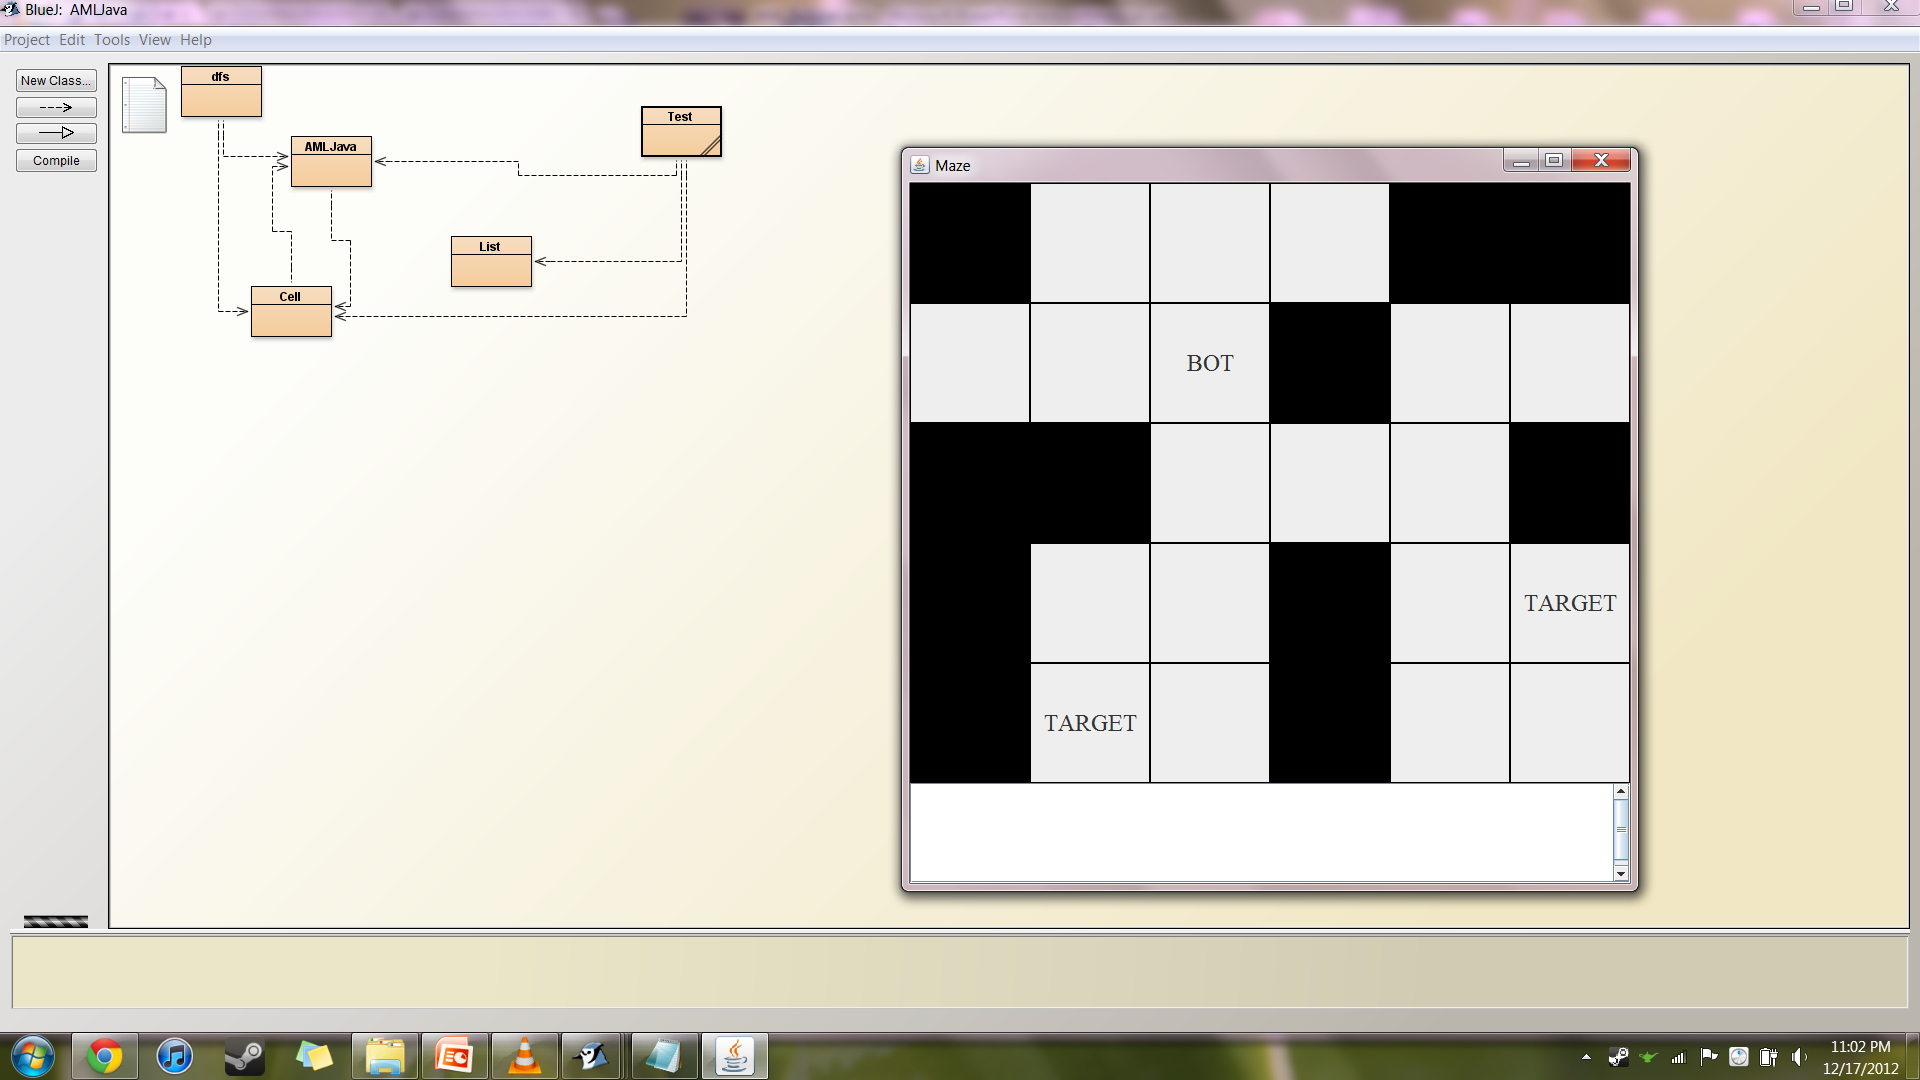
\includegraphics[height=80mm]{custommaze.png}
\caption{GUI representation of the text maze}
\end{figure}



\subsection{Example 1: Simple Program, Compilation}
Here is a very simple aML example:
\begin{center}
\begin{tabular}{c}
\begin{lstlisting}
#load-random

// function that is run by program initially
main():void {
	goRight();
}

function goRight():void {
	cell c := (CPos); // variables at start
	move_R(); // moves the bot to the right
	c := (CPos);
	if (NOT isTarget(c)) {
		goRight();
	}
} 
\end{lstlisting}
\end{tabular}
\end{center}

The first instruction in any aML program is the \#load instruction. This can either be \#load-random, which means aML will generate a random maze for you, or \#load<filename> which means you have a maze stored in filename.txt that you wish to be used. The main() function follows, and calls the recursive void function goRight(). goRight() instructs the bot to move right and check if the current cell (designated by the special variable CPos, standing for "current position") is the target. If not, it calls itself again. Obviously in most cases this bot will not be very effective and recurse endlessly (which amL will not stop from happening!), as in the case shown here:


\begin{figure}[htb]
\centering
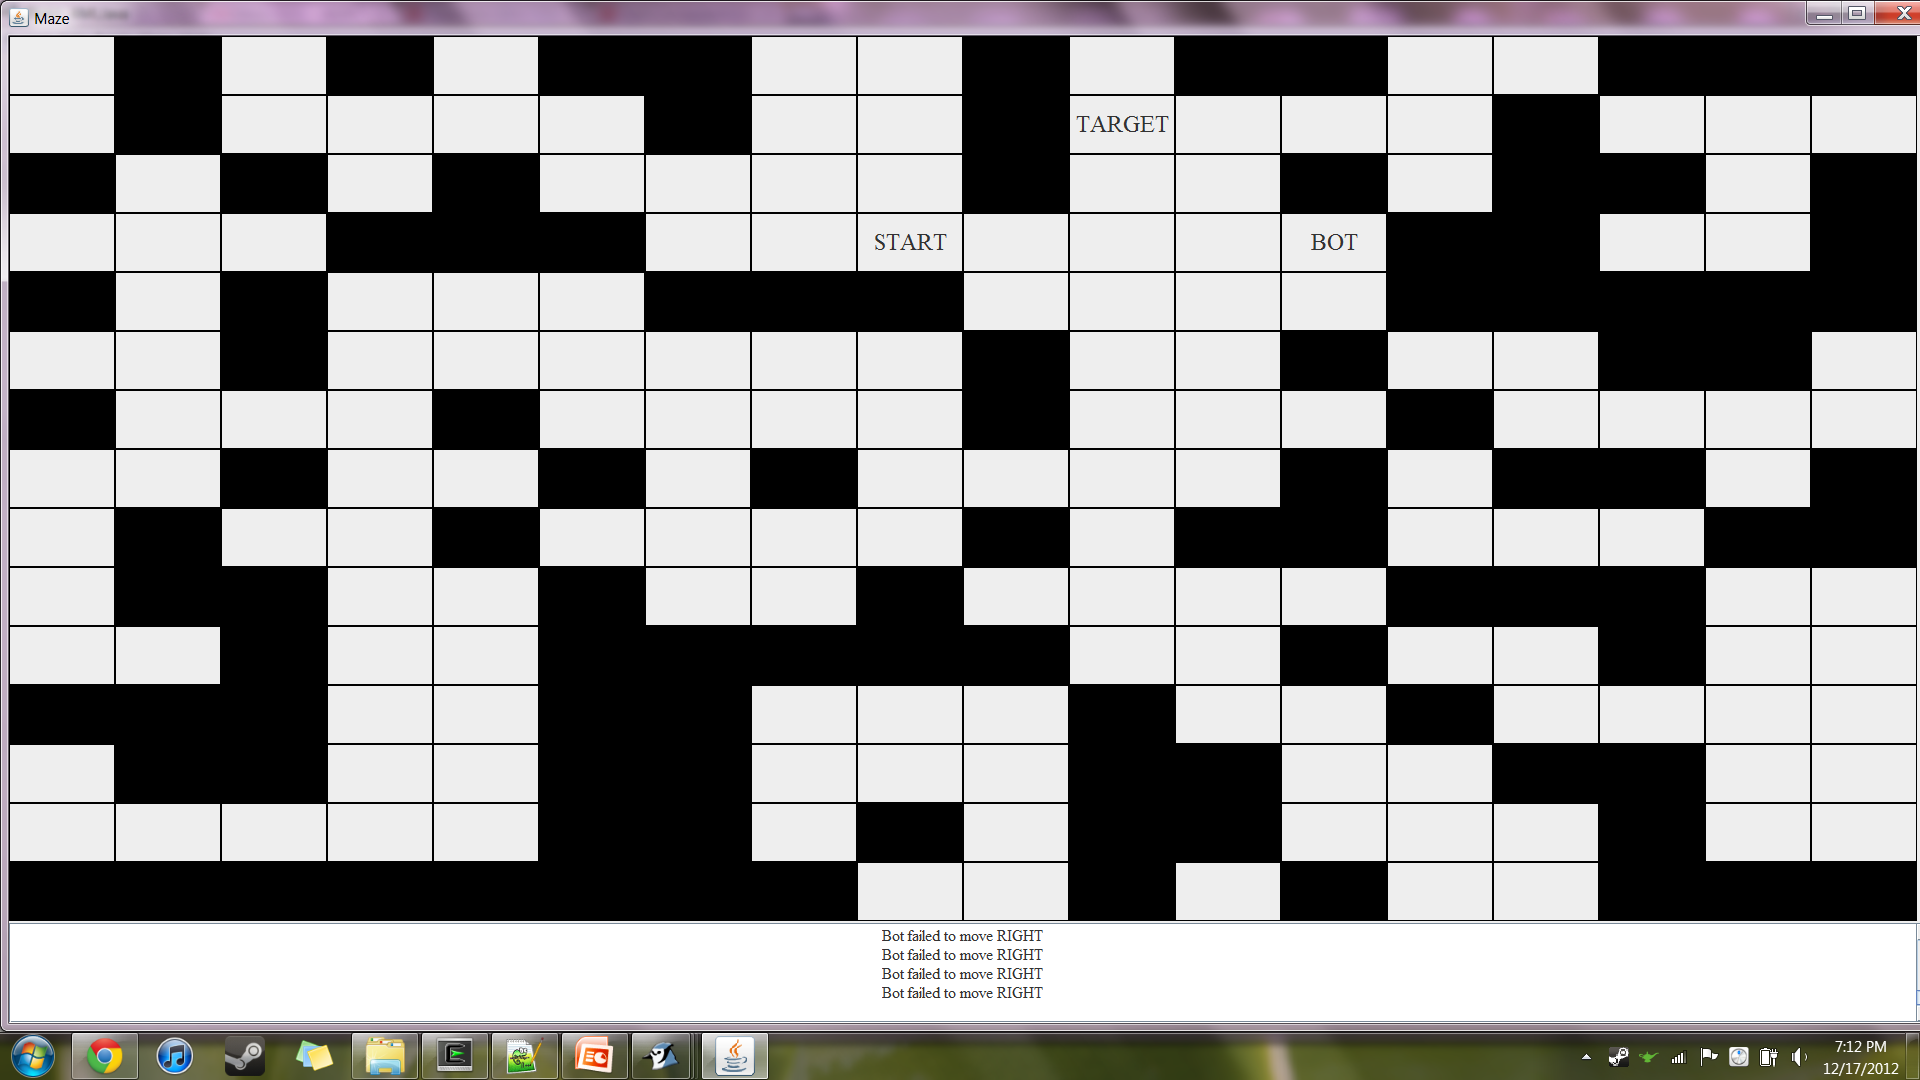
\includegraphics[height=80mm]{screenshot1.png}
\caption{GUI representation of the text maze}
\end{figure}


Another syntax rule in aML is that any variables in a function must be declared and initialized at the start of the function, prior to any other instructions. This is why cell c is initially set to a value before being reset after the use of the special move\_R() function (which instructs the bot to move right, if possible).

In order to compile an aML program, first construct aml.exe, which will compile the aML source code to an executable java program. In order to do this, use the provided makefile in the source files and simply type make into the command line. This will construct aml.exe. Then, if the example was in a file called example.aml, compile it by typing aml -c example.aml into the command line. This will construct a java program. Execute this by typing java example and the program will run.
	
	
\subsection{Example 2: Depth-First Search}
	It is possible to use aML to write much more complex functions than the first example. For example, here is a program that implements depth-first search:

\begin{lstlisting}
#load-random
main():void{
	DFS();
}



\end{lstlisting}


\begin{lstlisting}
function DFS():void{
	cell node := (CPos);
	
	if (isTarget(node)){
		exit();
	};
	
	if(myvisited(node)){
		DFS();
	};
	else{
		if (isSource(node)){
			exit();
		};

		revert();
		DFS();
	}
}



\end{lstlisting}


\begin{lstlisting}
function myvisited(cell node):bool{
	if (node.hasleft() AND NOT visited(node.left())){
		move_L();
	} else { if(node.hastop() AND NOT visited(node.up())){
		move_U();
	} else { if (node.hasright() AND NOT visited(node.right())) {
		move_R();
	} else { if(node.hasbottom() AND NOT visited(node.down())){
		move_D();
	} else {
		return false;
	}}}}
	return true;
}



\end{lstlisting}



Note the use of special functions such as node.hasright(), node.right(), revert() (which backtracks) and visited(cell c).

\subsection{Example 3: Greatest Common Denominator}
aML can also be used to implement a  simple mathematical function such as greatest common denominator, as in the following:


\begin{lstlisting}
#load-random

main():void{
	integer x := gcd(7,49);
	print(x);
	exit();
}

function gcd(integer n, integer m):integer{
	if(n = m){
		return n;
	};
	else{
		if (n > m) {
			return gcd(n - m, m);
		}
		else{
			return gcd(m - n,n);
		};
	};
}
\end{lstlisting}



\pagebreak{}
\section{Language Reference Manual}


\subsection{Introduction}

This manual describes the aML language which is used for manipulating
mazes and is used to provide instructions to a bot traversing the
maze. \\
The manual provides a reliable guide to using the language. While
it is not the definitive standard, it is meant to be a good interpretation
of how to use the language. This manual follows the general outline
of the reference manual referred to in \textquotedblleft{}The C Programming
Language\textquotedblright{}, but is organized slightly differently
with definitions specific to aML. The grammar in this manual is the
standard for this language.


\subsection{Lexical Conventions}

A program consists of a single translation unit stored as a file.
There are five classes of tokens: \textbf{identifiers}, \textbf{keywords},
\textbf{constants}, \textbf{operators}, and other separators. White
space (blanks, tabs, newlines, form feeds, etc.) and comments are
ignored except as they separate tokens. Some white space is required
to separate adjacent identifiers, keywords, and constants.


\subsubsection{Comments}

The characters // introduces a single line comment. The rest of the
line is commented in this case. This differs from a multi-line comment
which is enclosed by the /{*} and {*}/ characters. Multi-line comments
do not nest.


\subsubsection{Identifiers}

An identifier is a sequence of letters and digits, beginning with
a letter and can be of any length. The case of the letters is relevant
in this case. No other characters can form identifiers. \\
eg. abcd, Abcd, A123,abc1


\subsubsection{Keywords}

The following identifiers are reserved for use as keywords, and may
not be used otherwise:-\\
\\
\begin{tabular}{ccccccc}
if & return & display & remove & left & hasleft & integer\tabularnewline
then & main & print & add & right  & hasright & bool\tabularnewline
else & void & isSource & head & up  & hastop & list\tabularnewline
load & function & visited & next & down & hasbottom & cell\tabularnewline
random & exit & isTarget & isEmpty & CPos &  & \tabularnewline
true & null & NOT & AND &  &  & \tabularnewline
false &  &  & OR &  &  & \tabularnewline
\end{tabular}\\
\\
This language consists of many implicit variables and functions increasing
the size of the reserved words list. There are a few keywords like
display,null and next whose functionalities are not defined yet. But
they are reserved for future use.


\subsubsection{Literals}

There are different kinds of literals (or constants) in aML as listed
below:-


\paragraph{integer Literals}

An integer literal is taken to be decimal, and is of data type integer.
It may consist only of a sequence of digits 0-9. \\
eg. 0,1,22,-5


\paragraph{bool Literals}

A bool literal is either \textbf{True} or \textbf{False}, and is of
data type bool


\paragraph{list Literals}

The list literal can include either the integer, bool, cell or list<datatype>
types (cascaded lists). \\
eg. <{[}1{]}>,<{[}1,2,3{]}>,<{[}{[}1,2,3{]},{[}4,5{]}>,<{[}true, false,
true{]}>\\
.\\
As can be seen above the list literals consist of the form list<integer>,
list<list<....<list<integer>\textcompwordmark{}>...>\textcompwordmark{}>,
list<bool> or list<list ... <list <bool>\textcompwordmark{}> ... >\textcompwordmark{}>.
Details on list<datatype> and cell datatypes are provided in section
\ref{sec:Implicit-variables-and}. \\



\subsubsection{Separators}

The semi-colon \textbf{; }and the pair of braces \textbf{\{ \} },
the < > and {[} {]}, act as separators of the tokens. They are meant
to reduce ambiguity and conflicts during the parsing phase. The semi-colon
is added at the end of every statement to signify the end of the logical
statement. The \{ \} are used to collect groups of statements into
a single compound statement block. The < > and {[} {]} are used to
instantiate the list<datatype> variables.


\subsection{Syntax Notation}

In all of the syntactic notation used in this manual, the non-terminal
symbols are denoted in \textit{italics}, and literal words and characters
in \textbf{bold. }Alternative symbols are listed on separate lines.
An optional terminal or non-terminal symbol is indicated by subscripting
it with 'opt'. \\
eg. \textit{expression\textsubscript{opt}} denotes an optional expression


\subsection{Identifier interpretation}

aML interprets the identifier based on it's type. Each identifier
has a storage associated with it where a certain value is stored.
The type of the identifier determines the meaning of the values located
in the storage of the identifier. In aML each identifier's storage
exists as long as the block enclosing the identifier is being executed.\\
aML supports a 3 fundamental types:-\\

\begin{itemize}
\item integer - Objects declared as integers use 64 bits for storage and
are signed. They are primarily used for arithmetic operations.
\item bool - Objects declared as bools act as binary variables and can either
take the value \textbf{true} or \textbf{false}.
\item cell - A cell object stores the attributes of a cell of a maze.
\end{itemize}
There is one derived type list<type> which is used for storing lists
of objects of the fundamental types as well as the list type. By this
recursive definition, aML allows cascading of these lists.\\
 More details on the cell and list<type> datatypes is provided in
section \ref{sec:Types-revisited}.\\
\\
The complete data type definitions present in aML are as follows:-\\
\textit{}\\
\textit{datatype:-}\textbf{}\\
\textbf{\hspace*{0.5cm}integer}\\
\textbf{\hspace*{0.5cm}bool}\\
\textbf{\hspace*{0.5cm}cell}\\
\textbf{\hspace*{0.5cm}list<}\textit{datatype>}\\
\\
\textbf{Note:- }Each datatype is different from each other and no
two different datatypes can be combined together in a valid operation
defined in aML. Therefore there are no type-conversion rules defined
for aML.


\subsection{Expressions}

The complete syntax is provided in section \ref{sec:Syntax-summary}.
This section introduces the definition of the expression types which
are the basic building blocks of any language.


\subsubsection{Primary Expressions}

Primary expressions are identifiers, constants, or expressions in
parentheses. They also include the variable CPos which will be explained
in section \ref{sec:Types-revisited}.\\
\textbf{}\\
\textit{primary-expression:-}\\
\textit{\hspace*{0.5cm}identifier}\\
\textit{\hspace*{0.5cm}literal }\\
\textit{\hspace*{0.5cm}}( \textit{expression }\textbf{)}\textbf{\textit{}}\\
\textit{\hspace*{0.5cm}}\textbf{(CPos)}\\
 \\
An identifier is a primary expression provided it's type is specified
in it's declaration.\\
A literal is a primary expression. The type of the literal may include
integer, bool or list<type>. The syntax notation for literal including
the definition of list literals is given in detail in section \ref{sec:Syntax-summary}.
\\
A paranthesized expression is a primary expression whose type and
value are equal to those of the non-paranthesized one. \\
CPos refers to the current position of the bot in the maze. It is
a tracking variable and is used primarily to assign values to identifiers
of cell datatypes. \\
null is a constant which is assigned by default to identifiers of
the list<type> and cell datatypes. It signifies no storage allotted
to the identifier yet.


\subsubsection{Operators}


\paragraph{Arithmetic Operators}

There are six arithmetic operators:\{ +, -, {*}, /, \%, \textasciicircum{}\}.
The operands of these operators must be of integer data type. The
result will also be of type integer.\\
\textbf{}\\
\textit{arithmetic-expression:-}\\
\textit{\hspace*{0.5cm}expression + expression }\\
\textit{\hspace*{0.5cm}expression - expression }\\
\textit{\hspace*{0.5cm}expression {*} expression }\\
\textit{\hspace*{0.5cm}expression / expression }\\
\textit{\hspace*{0.5cm}expression \% expression }\\
\textit{\hspace*{0.5cm}expression \textasciicircum{} expression }\\
\\
\begin{tabular}{|c|c|c|}
\hline 
Operator & Semantic & Comments\tabularnewline
\hline 
\hline 
+ & addition & \tabularnewline
\hline 
- & subtraction & \tabularnewline
\hline 
{*} & multiplication & \tabularnewline
\hline 
/ & division & integer division only. Divide by zero => error\tabularnewline
\hline 
\% & modulo & \tabularnewline
\hline 
\textasciicircum{} & exponentiation & \tabularnewline
\hline 
\end{tabular}\\
\\



\paragraph{Relational Operators}

The relational operators all return values of bool type (either True
or False). There are six relational operators: \{==, \textasciitilde{}=,
>, <, >=, <=\}. The operators all yield \textbf{False} if the specified
relation is false and \textbf{True} if it is true. \\
\textbf{}\\
\textit{relational-expression:-}\\
\textit{\hspace*{0.5cm}expression}\textbf{\textit{ }}\textbf{== }\textit{expression}\\
\textit{\hspace*{0.5cm}expression}\textbf{ \textasciitilde{}= }\textit{expression}\\
\textit{\hspace*{0.5cm}expression}\textbf{ > }\textit{expression}\\
\textit{\hspace*{0.5cm}expression}\textbf{ < }\textit{expression}\\
\textit{\hspace*{0.5cm} expression}\textbf{ >= }\textit{expression}\\
\textit{\hspace*{0.5cm}expression}\textbf{ <= }\textit{expression}\\
\\
\begin{tabular}{|c|c|}
\hline 
Operator & Semantic\tabularnewline
\hline 
\hline 
== & equals\tabularnewline
\hline 
\textasciitilde{}= & not equals\tabularnewline
\hline 
> & greater\tabularnewline
\hline 
< & lesser\tabularnewline
\hline 
>= & greater than equals\tabularnewline
\hline 
<= & less than equals\tabularnewline
\hline 
\end{tabular}\\
\\
The \textbf{==} operator compares the value of left expression to
the right expression and evaluates to True if they are equal, False
otherwise. It is vice-versa for the \textbf{\textasciitilde{}= }operator.
The \textbf{> }operator evaluates to true if the left expression is
greater than the right expression, false otherwise. The \textbf{<
}operator behaves in the opposite manner. The \textbf{>= }and \textbf{<=
}operators check for equality condition as well. \\
For the == and \textbf{\textasciitilde{}= }operators, the expressions
involved must be of the same datatype. The other operators are defined
only for the integer datatype where comparison is meaningful. For
the cell datatype, the == and \textasciitilde{}= compare the cell
location in the map to which both the operands point to. As for the
list<type> datatype, the two operators check if two variables referencing
list datatypes point to the same list object.\\



\paragraph{bool Operators}

The bool operators all return values of bool type (either True or
False). There are three bool operators: logical-NOT, logical-AND and
logical-OR, denoted by NOT, AND, and OR, respectively. \\
\textbf{}\\
\textit{not-expression:-}\\
\textit{\hspace*{0.5cm}}\textbf{NOT}\textit{ expression}\\
\textit{and-expression:-}\\
\textit{\hspace*{0.5cm}expression }\textbf{AND}\textit{ expression}\\
\textit{or-expression:-}\\
\textit{\hspace*{0.5cm}expression }\textbf{OR}\textit{ expression}\\
\\
The operand(s) to NOT, AND and OR have to evaluate to True or False,
or in other words, they must either be bool variables or relational
expressions. NOT negates the operand, AND returns True if all operands
evaluate to true, False otherwise. OR returns True if at least one
of the operands evaluate to true, False otherwise.


\paragraph{Assignment Operators}

There is a single assignment operator in aML, \textbf{:=,} which does
simple assignment. It is a binary operator which assigns the value
of the right operand to the storage of the left operand.\\
\\
\textit{assignment-expression:-}\\
\textit{\hspace*{0.5cm}identifier }\textbf{:=}\textit{ expression}\\
\textit{}\\
The type of the expression must be identical to the type of 'lvalue'.


\paragraph{Associative Operator}

The \textbf{. }operator is used for function calls on variables represented
by identifiers. The structure of statements involving the operator
is shown in section\ref{sec:Syntax-summary}.


\subsection{Declarations}

Declarations specify the interpretation given to each identifier i.e.
the type of data it can point to and the associated operations that
go along with it. Declarations can be divided into variable and function
declarations. Variable declarations refers to the declaration of identifiers
whose type belongs to one of the datatypes mentioned and is different
from function declarations both syntactically and semantically.


\subsubsection{Variable Declarations\label{sub:Variable-Declarations}}

The rule representing the declaration of identifiers is listed in
the complete Syntax summary in section \ref{sec:Syntax-summary}.
The declaration of identifiers is similar to many strongly typed languages
where thet type associated with the identifier must be specified during
declaration. In aML variable declaration is allowed only at the beginning
of the main method and other functions. Without any loss of generality
variable declaration is not allowed to intermix with statements and
also it is encourage that while declaring variables at the top, they
are assigned to literal values initally, or function calls, but not
other variables. They can be assigned to subsequent variables using
assignment statements in the body of the function.\\
\\
\textit{declaration-expression:-}\\
\textit{\hspace*{0.5cm}datatype identifer := literal }\\
\textit{\hspace*{0.5cm}datatype identifier := }\textbf{(CPos)}\textit{
}\\
\textit{\hspace*{0.5cm}datatype identifier := lang\_functions}\\
\\
\\
Examples of some declarations are given below:-
\begin{itemize}
\item integer x;
\item bool flag;
\item cell node;
\item list<integer> mylist;
\end{itemize}

\subsubsection{Variable Initialization\label{sub:Variable-Initialization}}

When an identifier is declared, an initial value must also be specified.
The identifier can be re-initalized after it's declaration using assignment
statements. \\
 \textit{}\\
\textit{init-expression:-}\\
\textit{\hspace*{0.5cm}identifier} \textbf{:=} \textit{expression}\\
\\
Care must be taken to ensure that the identifer's type must be consistent
with the type of the expression.\\


A few examples of variable initializations are provided below;
\begin{itemize}
\item x := 10;
\item flag := false;
\item node := null;
\item mylist.head() := 1;
\end{itemize}
The exact rule is provided in the Syntax summary in section \ref{sec:Syntax-summary}.
Initialization can also be combined with declaration in a single step.
This is also shown in final section.


\subsubsection{Function Declaration}

Functions can either return a certain datatype or be void functions
(return no value). A function header is specified with the \textbf{function
}keyword and an identifier along with an optional argument list and
return type. Functions can be {}``used'' by function calls. But
for a function to be called, it must be declared in the program.\\
\\
\textit{function\_declaration:-}\\
\textit{\hspace*{0.5cm}function\_header}\textbf{ \{ }\textit{vdecl\_list
body}\textbf{ \}}\\
\textbf{}\\
\textit{function\_header:-}\\
\textit{\hspace*{0.5cm}}\textbf{function}\textit{ identifier (args\_list\textsubscript{\textbf{opt}})}\textbf{
: }\textit{return\_type}\\
\textit{}\\
\textit{args\_list:-}\\
\textit{\hspace*{0.5cm}datatype identifier}\\
\textit{\hspace*{0.5cm}datatype identifier}\textbf{,}\textit{ args\_list}\\
\textit{}\\
\textit{vdecl:}\\
\textit{\hspace*{0.5cm}datatype identifier := litera}\\
\textit{\hspace*{0.5cm}datatype identifier := }\textbf{(CPos)}\textit{
}\\
\textit{\hspace*{0.5cm}datatype identifier := lang\_functions}\\
\textit{}\\
\textit{vdecl\_list:}\\
\textit{\hspace*{0.5cm}empty declaration}\\
\textit{\hspace*{0.5cm}vdecl vdecl\_list}\\
\textit{}\\
\textit{body:-}\\
\textit{\hspace*{0.5cm}compound-statement}\textbf{}\\
\textbf{}\\
\textbf{}\\
Function calls are handled in section \ref{sec:Syntax-summary}. Compound
statements are described in detail in the section below. \\
Since function calls are part of compound statements, aML allows recursive
functions, which is necessary owing to the absence of any looping
constructs in this language. Also compound-statements do not allow
function definitions, so functions cannot be declared within functions.


\subsection{Statements}

Statements are usually executed in sequence, with the exception of
conditional statements. They are the next level of basic building
blocks after expressions. Each statement ends with a semi-colon at
the end which denotes the end of the logical statement. The physical
statement which is equivalent to one line in the editor may be comprised
of one or more logical statements.\\
One notable feature in aML is the lack of looping constructs. Iterations
are achieved by tail recursion of functions. The function definition
shown above is represented in the bigger picture in section \ref{sub:Program-Definition}.
The following definition gives an idea about the components of a statement.
The entire definition integrated with other definitions is present
in section \ref{sec:Syntax-summary}.


\subsubsection{Expression statement}

\textit{expression-statement:- }\\
\textit{\hspace*{0.5cm}expression}\textbf{;}\textit{ }\\
Expression statement consist of assignments and function calls. 


\subsubsection{Compound statements}

Compound statements are provided in the form:-\\
\\
 \textit{compound-statement:-}\\
\textit{\hspace*{0.5cm}}\textbf{\{ }\textit{statement-list }\textbf{\}}\textit{}\\
\textit{statement-list:-}\\
\textit{\hspace*{0.5cm}statement }\\
\textit{\hspace*{0.5cm}statement statement-list }\\
Compound statements are generally used to form the body of code to
execute in conditional statements, as well as the body of function
definitions.


\subsubsection{Conditional statements}

Conditional statements have the general form:-\\
\\
 \textit{conditional-statement:-}\textbf{}\\
\textbf{\hspace*{0.5cm}if }\textit{(expression)}\textbf{ then \{}\textit{compound-statement}\textbf{\};}\\
\textbf{\hspace*{0.5cm}if (}\textit{expression}\textbf{) then \{}\textit{compound-statement}\textbf{\}else
\{}\textit{compound statement}\textbf{\}}\\
\\
 The else branch is optional. The program will evaluate the expression
in parentheses, and if it evaluates to the bool value true then it
executes the corresponding compound-statement, and subsequently continues
on to the statement following the conditional statement. If the expression
does not evaluate to true, then the compound-statement following the
else branch is executed (if it exists). Branches are evaluated in
order, such that only the first branch with an expression that evaluates
to true will be executed, and all others skipped.


\subsubsection{Return statement}

Return statement Return statements take the form:-\\
\textit{return-statement:- }\\
\textit{\hspace*{0.5cm}}\textbf{return }\textit{expression}\textbf{;}\\
The expression should evaluate to a value of the return type of the
function being defined. 


\subsection{Scope rules}

Programs are not multi-file in AML, so external scope is not a worry.
The lexical scope of identifers is of relevance however. In brief,
subsequent to declaration a given identifier is valid for the rest
of the function inside which it was declared. Re-declarations using
an already declared identifier are not permitted. No identifiers can
be declared outside functions. \\
While user-defined variables cannot enjoy a global scope, the implicit
variables on the other-hand can do so. More information on implicit
variables is provided in \ref{sec:Implicit-variables-and}.


\subsection{Preprocessor directives}

Preprocessor directives must precede any code in the program. One
possible preprocessor directive takes the form: \textbf{\#load filename}.
This instruction ensures that the maze to be navigated is to be generated
from the file with name \textbf{filename}. (The file must be placed
in the 'maps' directory). The acceptable file format is pre-defined
and is independent of the language used. \\
Another possible directive is: \textbf{\#load-random}. This leads
to the maze is to be randomly generated each time the program runs.
\\
The two directives are mutually exclusive. In the event of multiple
directives, the compiler will show an error. 


\subsection{Implicit identifiers and functions\label{sec:Implicit-variables-and}}

aML consists of many implicit identifers or variables and functions.
By implicit, it follows that these identifiers can be used without
prior declaration as is the case for any user defined identifier or
function. However they cannot be modified by the user. Their usage
is mostly restricted to bool queries and assigning their values to
user-defined identifiers. The variables and functions along with their
meaing are provided below:-\\



\subsubsection{Variables}

The implicit variables are as follows.\\

\begin{itemize}
\item CPos - denotes the current position of the bot on the maze. Variables
of type cell can be instantiated by referencing CPos.
\item Visited - It is a dictionary like structure which maintains the 'visited'
status of each cell of the maze. It is used especially for backtracking
algorithms. It can never be used. The Visit() function provided accesses
this data structure inherently.
\end{itemize}

\subsubsection{Functions}

The implicit functions mainly deal with the movement and functionalities
of the bot. \\

\begin{itemize}
\item move\_U() - moves the bot one cell up from the current position, returns
true if it succeeds, false otherwise
\item move\_D() - moves the bot one cell down from the current position,
returns true if it succeeds, false otherwise
\item move\_L() - moves the bot one cell left of the current position, returns
true if it succeeds, false otherwise
\item move\_R() - moves the bot one cell right of the current position,
returns true if it succeeds, false otherwise
\item revert() - goes back to the previous position from the current position,
returns true if successful, false if at the start
\item visited(id) - checks if the cell refered to by id has been visited
or not
\end{itemize}

\subsection{Types revisited\label{sec:Types-revisited}}

This section discusses the list<datatype> datatype and the functions
associated with it. These two datatypes are in a sense less primitive
than the integer and bool datatypes. They come along with certain
functions which can be applied to variables belonging to these datatypes.
These functions are invoked or called using the \textbf{. }associative
operator on the identifier. The rule regarding the functions is shown
in the final section.


\subsubsection{list<datatype>}

The list<datatype> from it's definition in section\ref{sub:Variable-Declarations}
allows cascaded lists. This is especially useful for adjacency list
representation of graphs from mazes.\\
The functions associated with the datatype allow the manipulation
and traversal of the lists.\\

\begin{itemize}
\item add() - adds an elements to the end of the current list\\
eg. mylist.add(2);
\item remove() - removes and returns the first element of the current list\\
eg. mylist.remove();
\item isEmpty() - returns true if the current list has no elements, false
otherwise. \\
eg. mylist.isEmpty()
\item head() - returns the first element of the current list\\
eg. mylist.head();
\end{itemize}

\subsubsection{cell}

The cell datatype is unique in the sense that it cannot be set a user-defined
value. At any point of time, a variable of cell dataype can be assigned
only to the CPos value. It can however be stored in a variable which
will reflect that CPos value then, even if accessed at a later time.
\\
Certain functions are provided for this datatype which makes querying
the cell's content as well as it's neighborhood easier.


\paragraph{Neighborhood functions}
\begin{itemize}
\item left() - returns the left cell of the current cell if it exists and
the current cell has been visited
\item hasleft() - returns True if there is a cell to the left of the current
cell
\item right() - returns the right cell of the current cell if it exists
and the current cell has been visited
\item hasright() - returns True if there is a cell to the right of the current
cell
\item up() - returns the cell located upwards of the current cell if it
exists and the current cell has been visited
\item hasTop() - returns True if there is a cell to the top of the current
cell
\item down() - returns the cell located downwards of the current cell if
it exists and the current cell has been visited
\item hasbottom() - returns True if there is a cell to the bottom of the
current cell
\end{itemize}

\paragraph{cell functions}
\begin{itemize}
\item isTarget(id) - returns true if the cell is a target as specified in
the maze
\item isSource(id) - returns true if the cell is the start point of the
maze
\item get\_Loc(id) - returns the integer ID of the cell
\end{itemize}
Here id refers to an identifer pointing to a cell datatype.


\subsection{Syntax summary\label{sec:Syntax-summary}}

The entire syntax is provided below. This section is intended for
the logical understanding of the language structure rather than an
exact copy of the language.\\



\subsubsection{Expressions}

The expression includes declaration statements as well.\\
\\
\textit{expression:-}\\
\textit{\hspace*{0.5cm}primary\_expression}\\
\textit{\hspace*{0.5cm}lval\_expression}\textbf{}\\
\textbf{\hspace*{0.5cm}NOT }\textit{expression}\\
\textit{\hspace*{0.5cm}expression binop expression}\\
\textit{\hspace*{0.5cm}functions}\\
\textit{}\\
\textit{primary-expression:-}\\
\textit{\hspace*{0.5cm}identifier}\\
\textit{\hspace*{0.5cm}literal }\\
\textit{\hspace*{0.5cm}}( \textit{expression }\textbf{)}\textbf{\textit{}}\\
\textit{\hspace*{0.5cm}}\textbf{(CPos)}\\
\textbf{}\\
\textit{literal:-}\\
\textit{\hspace*{0.5cm}primitive\_literal}\\
\textit{\hspace*{0.5cm}}\textbf{<{[}}\textit{list\_literal\textsubscript{opt}}\textbf{{]}>}\textit{}\\
\textit{}\\
\textit{primitive\_literal:-}\\
\textit{\hspace*{0.5cm}integer\_literal}\\
\textit{\hspace*{0.5cm}bool\_literal}\\
\textit{}\\
\textit{list\_literal:-}\\
\textit{\hspace*{0.5cm}sub\_list}\\
\textit{\hspace*{0.5cm}}\textbf{{[}}\textit{list\_literal}\textbf{{]}}\textit{}\\
\textit{\hspace*{0.5cm}list\_literal,}\textbf{{[}}\textit{sub\_list}\textbf{{]}}\textit{}\\
\textit{}\\
\textit{sub\_list:-}\\
\textit{\hspace*{0.5cm}primitive\_literal}\\
\textit{\hspace*{0.5cm}primitive\_literal,sub\_list}\\
\textit{}\\
\textit{init-expression:-}\\
\textit{\hspace*{0.5cm}declarator := expression}\\
\textbf{}\\
\textit{datatype:-}\textbf{}\\
\textbf{\hspace*{0.5cm}integer}\\
\textbf{\hspace*{0.5cm}bool}\\
\textbf{\hspace*{0.5cm}cell}\\
\textbf{\hspace*{0.5cm}list<}\textit{datatype}\textbf{>}\\
\textbf{}\\
\textit{binop:-}\textbf{}\\


\begin{tabular}{|cccc|c|}
\hline 
 & Operators &  &  & Associativity\tabularnewline
\hline 
\hline 
\textasciicircum{} &  &  &  & Right\tabularnewline
\hline 
/ & {*} & \% &  & Left\tabularnewline
\hline 
> & < & >= & <= & Left\tabularnewline
\hline 
== & \textasciitilde{}= &  &  & Left\tabularnewline
\hline 
NOT &  &  &  & Right\tabularnewline
\hline 
AND &  &  &  & Left\tabularnewline
\hline 
OR &  &  &  & Left\tabularnewline
\hline 
:= &  &  &  & Right\tabularnewline
\hline 
\end{tabular}\\
\\
The binop table shows the binary operators in the decreasing order
of precedence (top - bottom) along with their associativity which
gives the fashion in which they are grouped together.\\
\\
\textit{functions:-}\\
\textit{\hspace*{0.5cm}list\_functions}\\
\textit{\hspace*{0.5cm}cell\_functions}\\
\textit{\hspace*{0.5cm}maze\_functions}\\
\textit{\hspace*{0.5cm}lang\_functions}\\
\textit{}\\
\textit{list\_functions:-}\textbf{}\\
\textbf{\hspace*{0.5cm}}\textit{identifier}\textbf{.remove()}\\
\textbf{\hspace*{0.5cm}}\textit{identifier}\textbf{.isEmpty()}\\
\textbf{\hspace*{0.5cm}}\textit{identifier}\textbf{.head()}\\
\textbf{}\\
\textit{cell\_functions:-}\textbf{}\\
\textbf{\hspace*{0.5cm}}\textit{identifier}\textbf{.left()}\\
\textbf{\hspace*{0.5cm}}\textit{identifier}\textbf{.right()}\\
\textbf{\hspace*{0.5cm}}\textit{identifier}\textbf{.up()}\\
\textbf{\hspace*{0.5cm}}\textit{identifier}\textbf{.down()}\\
\textbf{\hspace*{0.5cm}}\textit{identifier}\textbf{.hasleft()}\\
\textbf{\hspace*{0.5cm}}\textit{identifier}\textbf{.hasright()}\\
\textbf{\hspace*{0.5cm}}\textit{identifier}\textbf{.hastop()}\\
\textbf{\hspace*{0.5cm}}\textit{identifier}\textbf{.hasbottom()}\\
\textbf{\hspace*{0.5cm}isTarget(}\textit{identifier}\textbf{)}\\
\textbf{\hspace*{0.5cm}isSource(}\textit{identifier}\textbf{)}\\
\textbf{}\\
\textbf{}\\
\textit{maze\_functions:-}\\
\textit{\hspace*{0.5cm}}\textbf{visited}(\textit{identifier}\textbf{)}\\
\textbf{\hspace*{0.5cm}get\_Loc(}\textit{identifier}\textbf{)}\\
\textit{}\\
\textit{lang\_functions:-}\\
\textit{\hspace*{0.5cm}identifier}\textbf{(}\textit{actual\_args\textsubscript{\textbf{opt}}}\textbf{)}\\
\textbf{}\\
\textit{actual\_args:-}\\
\textit{\hspace*{0.5cm}primary\_expression}\\
\textit{\hspace*{0.5cm}primary\_expression}\textbf{, }\textit{actual\_args}\textbf{}\\
\textbf{}\\



\subsubsection{Statements}

Statements are logical sentences that can be formed by the language.
A compound statement is a group of statements occuring in a linear
fashion one after the other.\\
\textit{compound-statement}:\textbf{-}\\
\textbf{\hspace*{0.5cm}\{}\textit{statement-list}\textbf{\}}\\
\textbf{}\\
\textit{statement-list:-}\\
\textit{\hspace*{0.5cm}statement}\\
\textit{\hspace*{0.5cm}statement statement-list}\\
\textit{}\\
\textit{statement:-}\textbf{}\\
\textbf{\hspace*{0.5cm}}\textit{expression}\textbf{;}\\
\textbf{\hspace*{0.5cm}return }\textit{expression}\textbf{;}\\
\textbf{\hspace*{0.5cm}\{ }\textbf{\textit{statement-list}}\textbf{
\}}\\
\textbf{\hspace*{0.5cm}if (}\textit{expression}\textbf{) }\textit{statement}\textbf{;}\\
\textbf{\hspace*{0.5cm}if (}\textit{expression}\textbf{) }\textit{statement}\textbf{
else }\textit{statement}\textbf{}\\
\textbf{\hspace*{0.5cm}exit();}\\
\textbf{\hspace*{0.5cm}print(}\textit{expression}\textbf{);}\\
\textbf{\hspace*{0.5cm}}\textit{move\_functions}\textbf{;}\\
\textbf{\hspace*{0.5cm}}\textit{lang\_functions}\textbf{;}\\
\textbf{\hspace*{0.5cm}}\textit{identifier}\textbf{.add(}\textit{expression}\textbf{);}\\
\textit{}\\
\textit{}\\
\textit{move\_functions:-}\textbf{}\\
\textbf{\hspace*{0.5cm}move\_To(}\textit{identifier}\textbf{)}\\
\textbf{\hspace*{0.5cm}move\_U()}\textit{}\\
\textbf{\hspace*{0.5cm}move\_D()}\textit{}\\
\textbf{\hspace*{0.5cm}move\_L()}\textit{}\\
\textbf{\hspace*{0.5cm}move\_R()}\textit{}\\
\textbf{\hspace*{0.5cm}revert()}\textit{}\\
\textbf{}\\
\\
If the expression to 'if' does not evaluate to True or False, an error
will be thrown. 


\subsubsection{Program Definition\label{sub:Program-Definition}}

This subsection describes the structure of the program and functions
which are the biggest building blocks in aML. Every aML must have
one and only one main function through which the control passes to
the program. It must also have exactly one pre-processor directive
to load the maze. It can have an arbitrary number of functions though.
The program structure is defined below:-\\
\\
\textit{program:-}\\
\textit{\hspace*{0.5cm}empty\_program}\\
\textit{\hspace*{0.5cm}pre-process program}\\
\textit{\hspace*{0.5cm}func-def program}\\
\textit{}\\
\textit{\hspace*{0.5cm}}\\
\textit{pre-process:-}\textbf{}\\
\textbf{\hspace*{0.5cm}\#load-}\textit{identifier}\textbf{}\\
\textbf{\hspace*{0.5cm}\#load-random}\\
\textbf{}\\
func-def:-\textbf{}\\
\textbf{\hspace*{0.5cm}main():void \{}\textit{vdecl\_list statement-list}\textbf{\}}\\
\textbf{\hspace*{0.5cm}function}\textit{ identifier}\textbf{(}\textit{formal-args\textsubscript{\textbf{opt}}}\textbf{):}\textit{return-type}\textbf{\{}\textit{vdecl\_list
statement-list}\textbf{\}}\\
\textbf{}\\
\textit{formal-args\textsubscript{\textbf{opt}}:-}\\
\textit{\hspace*{0.5cm}datatype identifier}\\
\textit{\hspace*{0.5cm}datatype identifier}\textbf{,}\textit{formal-args}\textbf{\textit{}}\\
\textbf{\textit{}}\\
\textit{return-type:-}\\
\textit{\hspace*{0.5cm}datatype}\textbf{}\\
\textbf{\hspace*{0.5cm}void}\\
\textbf{}\\
\textit{}\\
\textit{vdecl:}\\
\textit{\hspace*{0.5cm}datatype identifier := literal}\\
\textit{\hspace*{0.5cm}datatype identifier := }\textbf{(CPos)}\textit{
}\\
\textit{\hspace*{0.5cm}datatype identifier := lang\_functions}\\
\textit{}\\
\textit{vdecl\_list:}\\
\textit{\hspace*{0.5cm}empty declaration}\\
\textit{\hspace*{0.5cm}vdecl vdecl\_list}\\
\textit{}\\

\pagebreak

\section{Architecture Design}
aML was designed in such a fashion that the aML syntax was similar to the java syntax making the translation to java much easier. Hence java was chosen to be the language to be  translated to. The standard library functions were provided in java, where the maze was visualized using the java Swing GUI.


Keeping this in mind, the architecture of aML was designed as shown below tracing the steps from character streams typed by the user all the way to compiled java bytecode.



\begin{enumerate}
\item
The lexical analyzer accepts a character stream and converts into a token stream. These tokens are defined in scanner.mll - the set of acceptable words in our language.  The token stream is passed onto the Parser.
\item
The Parser ensures that the token stream input received is consistent with the grammar rules defined in parser.mly -- the order in which the tokens can combine with each other forming the syntax of the language.  The parser while checking for grammar rule consistency forms the Abstract Syntax Tree or AST, with the help of the ast structures defined in ast.ml. This incidentally also contains the one-one mapping of ast nodes to translated java code.  The ast structure is passed onto the Semantic Analyzer.
\item
The Semantic Analyzer ensures that the syntax is actually meaningful. It ensures that the program defined by the user while conforming to the grammar actually make sense. For example the assignment of variables to values, the semantic analyzer ensures that the types have to be consistent for this to be a valid operation. The semantic analysis for aML is present in sast.ml.
\item
Once the semantic analysis is done and successful without throwing any exceptions, the verified ast structure can be translated to a .java file and compiled to .class (java bytecode). This is done in the file compile.ml. 
\item
The file toplevel.ml is provided for the user's convenience to run the program using the command line interface. The exact usage is shown on typing ./aml in the command line.
\end{enumerate}


\pagebreak

\section{Test Plan}

For our test suite, we decided to include both unit and functional tests for maximum coverage of our language's features. Both are necessary because alone, these two types of testing give only a limited guarantee of correctness, but together they ensure that everything works how it is supposed to. Unit tests test individual features in isolation, for example the correct translation of the addition operator or a function declaration. These are important because before we can even hope to ensure that our full codebase works properly, we must ensure that each unitary component provides the correct output for a given input. Because we didn't want to accidentally omit a feature of our language from the unit tests, our strategy for writing unit tests was to go through the LRM and create a test case for each feature described therein.  

Functional tests are at the other end of the testing spectrum -- they validate not a simple input-to-output conversion, but rather the result of complex interactions between many parts of the code. An example functional test case could be something like a GCD algorithm or a simple search algorithm. The reason we need functional tests on top of unit tests is that there is no way to verify that the pieces of our code work properly \textit{together }if we use only unit testing, which verifies that the pieces of our code work properly \textit{apart}. 

We decided to implement and automate our tests using bash script. All of this can be found in the tests subdirectory. Each individual test case has two components: (1) an aML source file containing the aML code relevant to the test case, and (2) a bash script file of the same name (but with a .test extension rather than a .aml extension) that contains the expected output from the test case as well as any other necessary information pertaining to the test case in question (for example, setting COMPILE\_ONLY=true if the test case is meant to cause an error on compilation). The bash file "test-base" contains all the functions necessary for automating the testing process, including functions to compile and run an individual test case, to print error/info data to the console, and to run the full suite at one time.


\pagebreak


\section{Lessons Learned}
\begin{itemize}
\item
One of the things that we learned is that a group should always start
early so that there is time to work out issues before deadlines. By
starting a little earlier on some sections, we may have been able to
avoid having to rush to fix certain issues before parts of the project
were due.
\item
Another thing we learned is the need to be flexible with your ideas
and not plan for a lot of features too early. A good approach would
have been to start simple and build off of simple features as we move
along. Planning for too many features caused us to have to change our
thinking at certain points during the project.
\end{itemize}



\subsection{Sriramkumar Balasubramanian}
\begin{itemize}
\item
Keep in frequent communication.
\item
Start earlier than you will.
\item
Spread the work out.
\item
Sleepless coding is inefficient and/or error-prone.

\end{itemize}
\subsection{Evan Drewry}
\begin{itemize}
\item
Being super organized is a very important factor in coding project as a team, especially when the team isn't always working together in the same room. Lack of organization can lead to confusion or wasted time for other group members who are also working on the project.
\item
Testing incorrect programs is as important as testing correct ones. If we only included meaningful and well-formed programs in our test suite, we would have no guarantee that our compiler responds appropriately to malformed input. Instead, we would only know that it respond appropriately to correct input.
\end{itemize}


\subsection{Tim Giel}
\begin{itemize}
\item
I learned that it is incredibly difficult to find a suitable time for everyone in a group to meet, especially 
when there are more people.  With everyone's schedule constantly changing and workloads piling up as the semester went on, it became increasingly difficult to find a time for everyone.  Fortunately, we were all pretty flexible and were able to meet as a group a lot which definitely helped in getting to know one another and how each of us work, which helped us work on our project more efficiently.
\item
I also learned that it is very tough when you don't have as much programming experience as others.  While we all were essentially learning two new languages (aML and OCaml), my lack of experience made me have to work a little harder than the other group members I think.
\end{itemize}



\subsection{Nikhil Helferty}
\begin{itemize}
\item
Keep in frequent communication.
\item
Start earlier than you will.
\item
Spread the work out.
\item
Sleepless coding is inefficient and/or error-prone.

\end{itemize}


\pagebreak{}

\section{Appendix}

\subsection{ast.ml}
\lstset{
language=[Objective]Caml,
basicstyle=\color{MidnightBlue}\footnotesize\ttfamily, % print whole listing small
keywordstyle=\color{violet}\bfseries,
% underlined bold black keywords
identifierstyle=\color{black}, % nothing happens
commentstyle=\color{white}, % white comments
}
\begin{lstlisting}[caption=ast.ml]
type binopr = Add | Sub | Mul | Div | Mod | Eql | Neq | Lsr
| Leq | Gtr | Geq | Pow | And | Or | Not

type assoc = Remove| Next | Head | Empty | Up | Down | Left
| Right | Hleft | Hright | Htop | Hbtm 

type datatype = 
    Integer 
| Bool 
| Cell
| List of datatype  

type return_type = 
    Void
| Data of datatype

type formal_args = FormalVar of datatype * string 

type vars = 
    Lit_Int of int
| Lit_Bool of bool
| Lit_List of vars list

type expr = 
    Id of string
| Vars of vars
| Paran of expr
| BinOpr of binopr * expr * expr
| Assoc of assoc * string
| Assign of string * expr
| Funcall of string * expr list
| Loc of string
| Target of string
| Src of string
| Visit of expr
| Pointer
| Null

type vdecl = 
    Define of datatype * string * expr

type stmt = 
    StmtBlk of stmt list
| Expr of expr
| Display
| Move of int
| MoveTo of string 
| Exit
| Revert
| Print of expr
| Return of expr
| ListAdd of string * expr
| If of expr * stmt * stmt

type main = {
    mainId : string;
    mainVars : vdecl list;
    body : stmt list; 
}

type func = {
    funcId : string;
    formalArgs : formal_args list;
    reType : return_type;
    localVars : vdecl list;
    statements : stmt list;
}

type funcs = 
    Main of main
| Func of func
| Load of string 

type program = 
    funcs list 

let string_of_dt = function
    Integer -> "int"
| Cell -> "Cell"
| List(e) -> "List "
| Bool -> "Boolean"

let string_of_assoc = function
    Remove -> "remove" 
| Next -> "clear" 
| Head -> "peek"
| Empty -> "isEmpty"
| Up  -> "up"
| Down -> "down"
| Left -> "left"
| Right -> "right"
| Hleft -> "hasLeft"
| Hright -> "hasRight"
| Htop -> "hasTop"
| Hbtm -> "hasBottom"

let rec string_of_rt = function
    Void -> "void"
| Data(e) -> string_of_dt e

let string_of_op = function
    Add -> "+" 
| Sub -> "-" 
| Mul -> "*" 
| Div -> "/"
| Eql -> "==" 
| Neq -> "!="
| Lsr -> "<" 
| Leq -> "<=" 
| Gtr -> ">" 
| Geq -> ">=" 
| Pow -> "^"
| Mod -> "%"
| And -> "&&"
| Or -> "||"
| Not -> "!"

let rec evalListexpr = function
    | [] -> ""
    | hd::[] -> string_of_var hd
    | hd::tl -> string_of_var hd ^ "," ^ evalListexpr tl 
and string_of_var = function
    | Lit_Int(f) -> string_of_int f
    | Lit_Bool(f) -> string_of_bool f
    | Lit_List(f) -> 
    	"new List( new Object [] {" ^ evalListexpr f ^ "})"

let rec string_of_expr = function
    Vars(e) ->
        string_of_var e
    | Id(s) -> s
    | BinOpr(o, e1, e2) ->
            begin
                match o with 
                | Pow -> "Math.pow(" ^ string_of_expr e1
                ^ " , " ^ string_of_expr e2 ^ ")"
                | Not -> "!" ^ string_of_expr e1
                | _ -> string_of_expr e1 ^ " " ^ (match o with
                  Add -> "+" | Sub -> "-" | Mul -> "*" | Div -> "/"
                | Eql -> "==" | Neq -> "!="
                | Lsr -> "<" | Leq -> "<=" | Gtr -> ">"
                | Geq -> ">=" | And -> "&&" | Or -> "||"
                | Mod -> "%"| Pow -> "^" | Not -> "!")  
                        ^ " " ^ string_of_expr e2
            end
                | Assign(v, e) -> v ^ " = " ^ string_of_expr e
                | Funcall(f, el) -> f ^ "(" 
                    ^ String.concat ", " 
                    (List.map string_of_expr el) ^ ")"
                | Assoc(f, e) ->  begin
                    match f with
                    | Remove ->"(Cell)"^ e ^ "."
                    	^ string_of_assoc f ^"()"
                    | Next -> e ^ "." 
                    	^ string_of_assoc f ^"()"
                    | Head -> "(Cell)"^ e ^ "."
                    	^ string_of_assoc f ^"()"
                    | Empty -> e ^ "."
                    	^ string_of_assoc f ^"()"
                    | _ ->  "AMLJava."
                    	^ string_of_assoc f ^"()"
            end
                    | Paran(e1) -> " ( " ^ string_of_expr e1 ^ " ) " 
                    | Loc(e) -> e^".get_Loc()"
                    | Target(e) -> e^".isTarget()"  
                    | Src(e) -> e^".isSource()"
                    | Visit(e) -> string_of_expr e ^ ".getVisited()"
                    | Pointer -> "AMLJava.current"
                    | Null -> "null"

let rec string_of_stmt = function
    StmtBlk(stmts) -> "{\n"
    ^ String.concat "" (List.map string_of_stmt stmts) ^ "}\n"
        | Expr(expr) -> string_of_expr expr ^ ";\n";
        | ListAdd(s,t) ->  s ^ ".add(" ^ string_of_expr t ^ ");\n"
        | Move(e) -> 
            begin
                match e with 
                | 1 -> "AMLJava.move_U();\n"
                | 2 -> "AMLJava.move_D();\n"
                | 3 -> "AMLJava.move_R();\n"
                | 4 -> "AMLJava.move_L();\n"
                | _ -> ""
            end
                | Exit -> "return;\n"
                | Revert -> "AMLJava.revert();\n"
                | Display -> "AMLJava.display();\n"
                | Print(e) -> "System.out.println (("
                    ^  string_of_expr e ^ "));\n"
                | Return(expr) -> "return "
                	^ string_of_expr expr ^ ";\n";
                | If(e, s, StmtBlk([])) -> "if ("
                	^ string_of_expr e
                    ^ ")\n" ^ string_of_stmt s
                | If(e, s1, s2) ->  "if (" ^ string_of_expr e ^ ")\n"
                    ^ string_of_stmt s1
                ^ "else\n" ^ string_of_stmt s2
                | MoveTo(x) -> "AMLJava.move(" ^ x ^");\n"

let string_of_vdecl = function 
    Define(dtt, nm, v) ->  string_of_dt dtt ^ " " ^ nm ^ " = "
    ^ string_of_expr v ^ ";\n"

let string_of_fparam = function
    FormalVar(dt,s) -> string_of_dt dt ^ " " ^ s

let string_of_func (func) = 
    "Function name : " ^ func.funcId ^ "\n" ^ 
    "Formal Parameter(s) : " ^ String.concat ","
    (List.map string_of_fparam func.formalArgs) ^ "\n" ^
    "Return Type: " ^ "\n" ^ string_of_rt func.reType	

let string_of_fdecl  = function
    | Func(fdecl) -> 
            "\npublic static "^ string_of_rt fdecl.reType^" "
            ^ fdecl.funcId ^ "(" ^ String.concat ", " 
            (List.map string_of_fparam fdecl.formalArgs)
            ^ "){\n" ^
            String.concat "" 
            	(List.map string_of_vdecl fdecl.localVars) ^
            String.concat ""
            	(List.map string_of_stmt fdecl.statements) ^
            "}\n"
    | Main(fdecl) -> 
            String.concat "" (List.map string_of_vdecl fdecl.mainVars) ^
            String.concat "" (List.map string_of_stmt fdecl.body) ^
            "}\n"
    | Load(str) -> 
    	"public static void main(String[] args){\nAMLJava.buildMaze(\""
        ^ str ^"\");"

let string_of_program (funcs) prog_name = 
	"import java.util.*;\n\npublic class "
	^ prog_name ^ "{\n" ^ 
	(String.concat "\n" (List.map string_of_fdecl funcs)) ^ "}" 

\end{lstlisting}



\end{document}